\documentclass[10pt,twocolumn]{article}
\usepackage[margin=0.75in]{geometry}
\usepackage[T1]{fontenc}
\usepackage{lmodern,microtype,amsmath,amssymb,booktabs,graphicx,xcolor}
\usepackage[hidelinks]{hyperref}
\usepackage{xurl}
\usepackage{array}
\newcolumntype{L}[1]{>{\raggedright\arraybackslash}p{#1}}
\usepackage[numbers,sort&compress]{natbib}
\usepackage{tikz,pgfplots}
\pgfplotsset{compat=1.18}
\usetikzlibrary{arrows.meta,positioning,fit,calc}
% Okabe-Ito colours, safe for colour-blind readers
\definecolor{oiblue}{HTML}{0072B2}\definecolor{oiorange}{HTML}{E69F00}
\definecolor{oiverm}{HTML}{D55E00}\definecolor{oigreen}{HTML}{009E73}\definecolor{oigrey}{HTML}{666666}
% Written by scripts/paper_numbers.py. Do not edit by hand.
\newcommand{\numSpeedOfLightKmS}{299792.458}
\newcommand{\numMarsOneWayS}{660.86}
\newcommand{\numMarsRoundTripS}{1321.72}
\newcommand{\numMarsDistanceMillionKm}{198.1}
\newcommand{\numMarsPlaysAsS}{11.01}
\newcommand{\numMoonOneWayS}{1.3}
\newcommand{\numStationOneWayS}{0.25}
\newcommand{\numCrewFirstAtS}{300}
\newcommand{\numSpeedup}{60}
\newcommand{\numSustainN}{5}
\newcommand{\numSettleN}{10}
\newcommand{\numPlausibleSpoTwoLow}{50}
\newcommand{\numPlausibleSpoTwoHigh}{100}
\newcommand{\numWindowN}{60}
\newcommand{\numMinReadings}{15}
\newcommand{\numMinDrop}{2}
\newcommand{\numMinAgreement}{0.5}
\newcommand{\numHorizonS}{600}
\newcommand{\numControlHours}{7.8}
\newcommand{\numControlFalseSosRaw}{4}
\newcommand{\numControlFalseSosReject}{1}
\newcommand{\numControlFalseSosSettle}{0}
\newcommand{\numControlTrendWarnings}{2}
\newcommand{\numUwEvents}{6}
\newcommand{\numUwWarned}{6}
\newcommand{\numUwMedianLeadS}{97}
\newcommand{\numUwMinLeadS}{14}
\newcommand{\numUwMaxLeadS}{159}
\newcommand{\numHrLimitBpm}{72.9}
\newcommand{\numHrWorstFlaggedMinPerH}{0.39}
\newcommand{\numHeldoutWarned}{6}
\newcommand{\numHeldoutMedianLeadS}{97}
\newcommand{\numGridSize}{18}
\newcommand{\numGridAllowed}{6}
\newcommand{\numHeldoutRounds}{6}
\newcommand{\numHeldoutRoundsShipSetting}{6}
\newcommand{\numSpoTwoCaution}{95}
\newcommand{\numSpoTwoWarning}{93}
\newcommand{\numSpoTwoEmergency}{91}
\newcommand{\numQuietS}{60}
\newcommand{\numWindowPairs}{1770}
\newcommand{\numNowMedianN}{5}
\newcommand{\numUsualMinReadings}{600}
\newcommand{\numUsualRefreshS}{300}
\newcommand{\numUsualHours}{24}
\newcommand{\numUsualLowPct}{1}
\newcommand{\numUsualHighPct}{99}
\newcommand{\numGridWindowShort}{45}
\newcommand{\numGridWindowLong}{60}
\newcommand{\numGridDropLow}{1.5}
\newcommand{\numGridDropHigh}{2.5}
\newcommand{\numGridAgreeLow}{0.4}
\newcommand{\numGridAgreeHigh}{0.6}
\newcommand{\numGridMaxControlWarnings}{3}
\newcommand{\numUwMinutesMin}{14}
\newcommand{\numUwMinutesMax}{19}
\newcommand{\numUwPredAbsErrMedianS}{16.5}
\newcommand{\numUwPredAbsErrMaxS}{50}
\newcommand{\numUwPredShortN}{4}
\newcommand{\numUwPredLongN}{2}
\newcommand{\numUwPredLongMaxS}{16}
\newcommand{\numUwWarnNormalBandN}{1}
\newcommand{\numUwTrendBeforeCautionN}{2}
\newcommand{\numApneaHours}{8.2}
\newcommand{\numApneaSosN}{579}
\newcommand{\numApneaWarnedFirstN}{185}
\newcommand{\numApneaWarnedFirstPct}{32}
\newcommand{\numApneaMedianLeadS}{42}
\newcommand{\numApneaLookbackS}{120}
\newcommand{\numHrPeople}{15}
\newcommand{\numHrSustainS}{60}
\newcommand{\numHrGateMinPerH}{1}
\newcommand{\numHrLimitPercentile}{99.9}
\newcommand{\numTestCount}{236}
\newcommand{\numRecorderHours}{24}
\newcommand{\numWorkedReadingOne}{97.0}
\newcommand{\numWorkedReadingTwo}{96.8}
\newcommand{\numWorkedReadingThree}{96.5}
\newcommand{\numWorkedReadingFour}{96.4}
\newcommand{\numWorkedReadingFive}{96.0}
\newcommand{\numWorkedN}{5}
\newcommand{\numWorkedPairs}{10}
\newcommand{\numWorkedSlope}{-0.25}
\newcommand{\numWorkedAgreement}{1}
\newcommand{\numWorkedLevel}{96.5}
\newcommand{\numWorkedGap}{5.5}
\newcommand{\numWorkedTimeLeftS}{22}
\newcommand{\numWorkedDrop}{1}


\title{Who decides when Earth is minutes away?\\ Latency-aware decision support for crew health monitoring}
\author{The LIGHT-TIME team, NASA Space Apps Challenge 2026, Orillia, Ontario\\\small Draft of 15 November 2026. Authors, affiliations and contributions are still to be agreed.}
\date{}

\begin{document}
\maketitle
\begin{abstract}
% Outline row: abstract.tex. One paragraph, at most 250 words: problem, what was built, how it was checked,
% the headline numbers as macros, the main limit, where the code is.
At Mars, a report from a spacecraft takes minutes to reach Earth and a reply twice as long: on 14 November 2026 the one-way light time was \numMarsOneWayS~s and the round trip \numMarsRoundTripS~s. A flight surgeon on Earth cannot direct care for a vital sign that will turn dangerous sooner than that. We describe LIGHT-TIME, a crew health monitor built for the NASA Space Apps Challenge 2026. Its ship computer sets who acts, the flight surgeon on Earth or the crew medical officer, from the one-way light time, switching at \numCrewFirstAtS~s by design choice. It fits a Theil--Sen slope with an agreement gate to a falling blood-oxygen reading and compares the time left with the round trip. It discards implausible readings before judging bands or trends; no trained model decides. We replayed public recordings through the same rules. All \numUwEvents{} recordings of induced low oxygen in healthy volunteers were warned before the SOS, by a median of \numUwMedianLeadS~s (range \numUwMinLeadS--\numUwMaxLeadS~s), and settings chosen with each recording left out warned on \numHeldoutWarned{} of \numUwEvents. In most recordings a fixed band was already held, so the trend rule's main addition was the stated deadline. On a healthy \numControlHours-hour night the trust rules cut false SOS from \numControlFalseSosRaw{} to \numControlFalseSosSettle. The evidence is \numUwEvents{} laboratory events on Earth: it shows the parts work as designed, not that the system helps a crew. Code, tests and the scripts behind every number are in the project repository.
\end{abstract}

\section{Introduction}\label{sec:intro}
% Outline row: introduction.tex. ISS care is ground-directed; Mars light time; NASA's distance hazard and EIMO;
% alarm fatigue; the gap; four contributions in prose.

On the International Space Station, medical care is directed from the ground. Astronauts rely on real-time contact with medical providers in mission control, and most medical expertise and decision-making sit on Earth~\cite{russell2023cdss,sirek2021autonomy}. On board, care is given by the crew medical officer (CMO), a crew member for whom there is little time for medical training among everything else a mission demands~\cite{russell2023cdss}. The arrangement works because the delay is short.

At Mars it is not. The one-way light time alone is about 3 to 22 minutes, from the closest and farthest Earth--Mars distances~\cite{nssdcMars}, and across planned crewed trajectories it peaks at about 22 minutes~\cite{mcbrayer2022delay}. On 14 November 2026, the date of our demonstration mission, it is about 11 minutes (\numMarsOneWayS~s), and a question to Earth costs the round trip, twice that. NASA lists distance from Earth as one of the hazards of human spaceflight and expects crews bound for Mars to confront medical emergencies with minimal support from teams on Earth~\cite{hrpDistance}. Its plans for Earth-independent medical operations (EIMO) move onboard care progressively into the crew's hands as missions go further out~\cite{levin2023eimo,lemery2024eimo}.

Monitoring software will be part of that shift, but more alarms are not the answer. Bedside monitors in intensive care already raise so many alarms that staff suffer alarm fatigue, and a life-threatening event can be missed among them; in one large study most of the arrhythmia alarms that nurses annotated were false positives~\cite{drew2014alarm}. A crew of a few people with one CMO cannot absorb that. A monitor for deep space has to raise fewer alarms, and each one has to reach the person who can act on it in time.

What distance changes is who can act in time. NASA's NEEMO~16 analog mission ran a simulated medical emergency under a five-minute communication delay, and the crew member's safety was compromised by the delay between crew and flight surgeon~\cite{rader2013delay}. If a reading is falling and will reach a dangerous level within a couple of minutes, a flight surgeon whose answer is a round trip away, \numMarsRoundTripS~s at Mars on our date, cannot help, however good the data they receive. Frameworks for space medicine already describe autonomy that grows with distance and delay~\cite{levin2023eimo,cypko2025}. We did not find an open monitoring system that takes the light time as an input on every alert, compares it with how long the patient has, and says plainly who must act.

LIGHT-TIME, built for the NASA Space Apps Challenge 2026, is a small attempt at that, and this paper describes its decision layer and how we checked it. First, the ship computer sets who acts, Earth or the crew, from the one-way light time read from an ephemeris for the mission date; the switch point is a design choice, kept as one constant. Second, a time-left estimate built from a Theil--Sen slope and an agreement gate is compared with the round trip, so a warning says whether Earth can answer before the reading reaches its red line. Third, trust rules discard readings that cannot be believed before any band or trend is judged. Fourth, we replayed public physiological recordings, all from volunteers on Earth, through the same rules, report every event, and check the settings by leaving each recording out; the code, its tests and the scripts that produce every number in this paper are open. The evidence is small, and so is the claim: this is an engineering design with a first replay check, not a clinical validation.

\section{Related work}\label{sec:related}
% Outline row: related.tex. Autonomy frameworks; onboard decision support; wearables in flight; early warning
% from wearables; alarm design; operations under delay. Table 1 holds only systems whose sources were verified.

\paragraph{Autonomy frameworks.}
The idea that medical authority should move toward the crew as Earth gets further away predates this work. NASA's Exploration Medical Capability element defines EIMO as a process in which terrestrial assets keep pre-mission screening, planning and prevention while onboard care increasingly becomes the crew's responsibility~\cite{levin2023eimo}, and a NASA workshop report sets out the same transition for Lunar and then Martian missions~\cite{lemery2024eimo}. The Canadian Space Agency's expert group on deep-space healthcare framed Canada's possible role around autonomous care in space and on Earth~\cite{csaDeepSpace2019}. Cypko et al.\ propose four autonomy levels tied to mission distance and communication latency, from Earth orbit to deep space~\cite{cypko2025}. These works describe the levels. LIGHT-TIME computes which level applies from the current light time and shows it on every screen.

\paragraph{Onboard decision support.}
NASA's concept of operations for an exploration clinical decision support system (CDSS) describes a tool that helps the crew assess and diagnose conditions and decide responses when communication with the ground is delayed or absent, and that eases delayed communication with flight surgeons~\cite{krihak2021cdss}; a later analysis of preliminary data suggests such a system could improve mission outcomes~\cite{russell2023cdss}. Google and NASA have tested a proof-of-concept CMO digital assistant that suggests diagnoses from reported symptoms, to support the CMO or the flight surgeon~\cite{googleCmoDa2025}. The CSA's Connected Care Medical Module (C2M2) programme funds prototype medical modules built around an AI-based system that connects medical devices~\cite{csaC2M2}. A NASA workshop on artificial intelligence for space health recommended an automated, autonomous ``precision space health'' system to monitor and assess crew health~\cite{scott2023}. LIGHT-TIME is narrower than any of these. It makes no diagnosis and uses no trained model to decide anything; it watches a few vital signs, states a deadline and names who can meet it.

\paragraph{Wearables in flight and on Earth.}
The CSA Bio-Monitor, a smart shirt with a headband and a tablet application, records heart activity, blood pressure, breathing, skin temperature, blood oxygen saturation and activity on the ISS, and sends the data to the ground~\cite{csaBioMonitor}. LIGHT-TIME assumes a garment of this kind as its sensor. On Earth, smartwatch heart rate and step counts have flagged infection before symptoms by comparing each person with their own baseline~\cite{mishra2020}, and a real-time alerting system built on that idea ran in a prospective study~\cite{alavi2022}. The personal usual range in LIGHT-TIME borrows the idea of a per-person baseline, but shows it as context and raises no alarm from it (Section~\ref{sec:methods}).

\paragraph{Alarm design.}
In intensive care, most monitor alarms are false or not acted on~\cite{drew2014alarm,gorges2009alarm}, and in one unit a short delay before each alarm was presented would have removed many of the ones that staff ignored~\cite{gorges2009alarm}. LIGHT-TIME applies the same idea to a crew's monitor: a band counts only after it has held for \numSustainN{} readings, and nothing can alarm while the sensor settles after a dropout.

\paragraph{Operations under delay.}
NASA's review of analog missions under communication delay recommended visual indicators of the delay, such as a countdown until a message is received, and procedures that rely on onboard tools rather than contact with the ground~\cite{rader2013delay}. LIGHT-TIME shows every message with its time to landing and its earliest reply. A simulator study of crews managing medical events found that crews without a flight surgeon performed worse, and concluded that checklists alone are not enough for autonomous care~\cite{yule2023crew}. The delay is also not the only gap. Near solar conjunction, communication with a Mars crew can be disrupted for days to months~\cite{mcbrayer2022delay}, so LIGHT-TIME has a no-link mode in which the crew act alone and messages wait in a queue.

\begin{table*}[t]\centering\footnotesize
\caption{Systems nearest to LIGHT-TIME, as described in the cited source. ``n.d.'': not described in that source. Only systems whose sources we could open and check are listed.}\label{tab:related}
\begin{tabular}{@{}L{0.15\textwidth}L{0.13\textwidth}L{0.18\textwidth}L{0.11\textwidth}L{0.19\textwidth}L{0.11\textwidth}@{}}\toprule
System & What it is & Earth delay in the logic & Time left to a threshold & Role & Code public \\ \midrule
ExMC CDSS~\cite{krihak2021cdss,russell2023cdss} & NASA concept of operations & delay and loss of contact drive the design & n.d. & helps the crew assess, diagnose and decide & n.d. \\
CMO digital assistant~\cite{googleCmoDa2025} & proof of concept & named as the motivation & n.d. & supports the CMO or flight surgeon from reported symptoms & n.d. \\
C2M2~\cite{csaC2M2} & funded prototypes & autonomy far from Earth is the aim & n.d. & AI-based system connecting medical devices & n.d. \\
Bio-Monitor~\cite{csaBioMonitor} & smart shirt flown on the ISS & n.d. & n.d. & records vital signs and sends them to the ground & n.d. \\
Autonomy levels~\cite{cypko2025} & position paper & four levels by distance and latency & n.d. & framework, not software & n.d. \\
Smartwatch alerting~\cite{alavi2022} & prospective study on Earth & not applicable & n.d. & alerts on deviation from a personal baseline & open-source platform stated \\
LIGHT-TIME (this paper) & hackathon build & light time for the mission date sets who acts & yes, compared with the round trip & rules and statistics; advises, never decides & repository; public release pending \\
\bottomrule
\end{tabular}
\end{table*}

\section{System}\label{sec:system}
% Outline row: system.tex. Figures 1 and 2. Link model, the mode rule, role-based views, implementation.

% Figure 1. Three layers and the delayed link. Drawn in TikZ so it stays sharp and editable.
\begin{figure*}[t]\centering
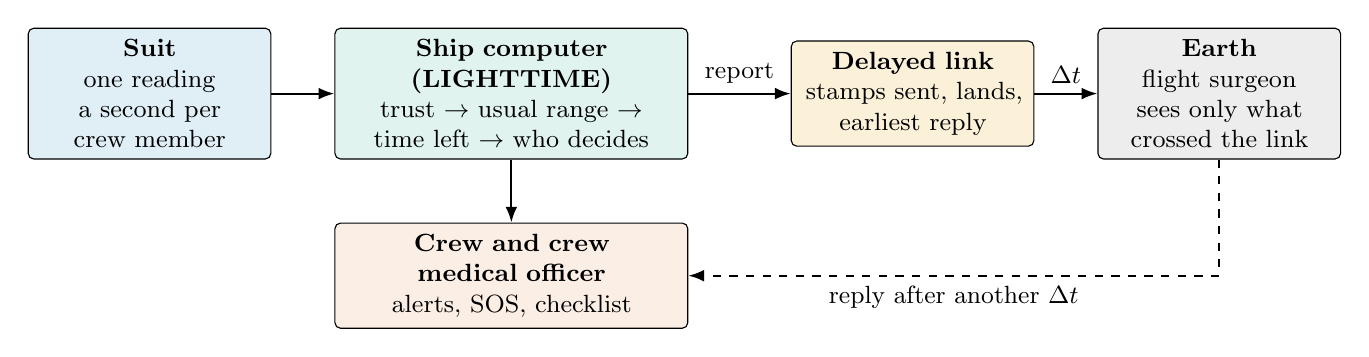
\begin{tikzpicture}[font=\small, box/.style={draw, rounded corners=2pt, align=center, minimum height=11mm, inner sep=4pt, text width=28mm},
  arr/.style={-{Latex[length=2mm]}, thick}]
\node[box, fill=oiblue!12] (suit) {\textbf{Suit}\\one reading a second per crew member};
\node[box, fill=oigreen!12, right=8mm of suit, text width=42mm] (ship) {\textbf{Ship computer (LIGHTTIME)}\\trust $\rightarrow$ usual range $\rightarrow$ time left $\rightarrow$ who decides};
\node[box, fill=oiorange!15, right=13mm of ship] (link) {\textbf{Delayed link}\\stamps sent, lands, earliest reply};
\node[box, fill=oigrey!12, right=8mm of link] (earth) {\textbf{Earth}\\flight surgeon sees only what crossed the link};
\node[box, fill=oiverm!10, below=8mm of ship, text width=42mm] (crew) {\textbf{Crew and crew medical officer}\\alerts, SOS, checklist};
\draw[arr] (suit) -- (ship);
\draw[arr] (ship) -- node[above]{report} (link);
\draw[arr] (link) -- node[above]{$\Delta t$} (earth);
\draw[arr] (ship) -- (crew);
\draw[arr, dashed] (earth.south) |- node[pos=0.75, below]{reply after another $\Delta t$} (crew.east);
\end{tikzpicture}
\caption{The three layers. The ship's rules set who acts from the one-way light time $\Delta t$; Earth reads only what has crossed the link.}
\label{fig:architecture}
\end{figure*}


LIGHT-TIME has three layers (Figure~\ref{fig:architecture}). A suit sends one reading a second for each crew member. The ship computer runs LIGHTTIME, the ship's rules and statistics, on every reading, keeps a recorder of the last \numRecorderHours~hours, and decides who must act. A delayed link carries reports to the flight surgeon on Earth and carries the replies back. We assume the crew wear a garment like the CSA Bio-Monitor, a smart shirt that the Canadian Space Agency flies on the International Space Station and that records heart activity, blood pressure, breathing, skin temperature, blood oxygen saturation and activity, including during sleep and exercise~\cite{csaBioMonitor}. We assume they wear it for the whole mission. That assumption matters for privacy, and we return to it in Section~\ref{sec:discussion}.

\paragraph{Suit hardware (design).}
The team designed its own sensor suit, a body-fitting skinsuit worn inside the spacecraft (Table~\ref{tab:suit}). An ESP32 DevKitC V4 board (ESP32-WROOM-32E) sits in a removable module at the front of the waist belt. The three I$^2$C sensors share GPIO21 (SDA) and GPIO22 (SCL) at 3.3~V with 4.7~k$\Omega$ pull-up resistors, and the board forwards timestamped records to the base station over Wi-Fi. Two readings need care: the MAX30205 measures skin temperature, which can differ from core body temperature, and the wearer's body shields the dosimeter at the back of the belt, so its placement would need calibration. The suit is a design and has not been built. The DevKitC is a development reference, and a flight version would need qualified hardware. The current ship software uses none of the EMG or motion data; those sensors are in the design for future rules. The hackathon build used a hobby pulse oximeter board as a stand-in sensor, the suit readings in the demo are simulated, and neither is part of the evaluation.

\begin{table*}[t]\centering\footnotesize
\caption{The suit as designed, not built. All wired sensors connect to the ESP32 through flexible wiring channels in the skinsuit. The current ship software reads none of the EMG or motion channels.}\label{tab:suit}
\begin{tabular}{@{}L{0.22\textwidth}L{0.25\textwidth}L{0.24\textwidth}L{0.21\textwidth}@{}}\toprule
Sensor & Measures & Interface to the ESP32 & Placement \\ \midrule
ESP32 DevKitC V4 (ESP32-WROOM-32E) & controller; forwards timestamped records over Wi-Fi & hub: I$^2$C on GPIO21 (SDA) and GPIO22 (SCL), 3.3~V, 4.7~k$\Omega$ pull-ups & removable module, front of the waist belt \\
DFRobot Gravity SEN0518 (MAX30102) & heart rate (beats a minute) and SpO$_2$ (\%) & I$^2$C & fingertip contact \\
MAX30205 & skin temperature ($^\circ$C) & I$^2$C & upper chest \\
GY-521 (MPU6050) & 3-axis acceleration and 3-axis rotation & I$^2$C & torso \\
Two MyoWare 2.0 EMG sensors~\cite{myowareSpecs} & muscle activation (EMG envelope) & analog, GPIO34 and GPIO35 & dominant-arm biceps; quadriceps \\
SPACEDOS02 dosimeter~\cite{spacedos02} & radiation measurement records; dose only after calibration & UART2 on GPIO16 and GPIO17; own battery & back of the waist belt \\
Upper-arm blood-pressure cuff & systolic and diastolic pressure (mmHg) & Bluetooth Low Energy & upper arm, at scheduled check-ins, not continuous \\
\bottomrule
\end{tabular}
\end{table*}

\paragraph{Light time and the link.}
The one-way light time is the time a signal needs to cover the distance between Earth and the ship:
\begin{equation}\label{eq:lighttime}
  \Delta t = \frac{d}{c},
\end{equation}
where $d$ is the path length in km and $c = \numSpeedOfLightKmS$~km\,s$^{-1}$ is the speed of light, exact by definition~\cite{bipmSI}, so $\Delta t$ is in seconds. For Mars the ship does not compute $d$ itself. It asks NASA JPL Horizons for the one-way light time from the centre of the Earth to Mars on the mission date~\cite{giorginiHorizons}. On our mission date, 14 November 2026, Horizons gives $\Delta t = \numMarsOneWayS$~s, about 11 minutes; multiplying back by $c$ gives $d = \numMarsDistanceMillionKm$~million km. A report and its answer each cross the link once, so the earliest possible reply comes one round trip after the report is sent:
\begin{equation}\label{eq:roundtrip}
  R = 2\,\Delta t ,
\end{equation}
which on our date is $R = \numMarsRoundTripS$~s, about 22 minutes. If Horizons cannot be reached, the ship falls back on values read from it the day before and labels them with that date. The two nearer stops of the demo use fixed delays: $\Delta t = \numStationOneWayS$~s for a station in low Earth orbit and $\Delta t = \numMoonOneWayS$~s for the Moon. Over a real Mars mission the one-way light time moves between about 3 and 22 minutes as the planets move~\cite{nssdcMars,mcbrayer2022delay}.

Every message between ship and Earth is a row in one table with the time it was sent, its delay and the time it lands. The other side cannot read a message until its landing time has passed, so the Earth console shows only what the link has delivered. Each message also carries the earliest time a reply could arrive, $R$ after it was sent. The Earth side of the code may read only that table and the position of the distance dial; a test fails if it imports any of the ship's crew, reading, alert, check-in or reminder tables. When there is no link, messages wait in a queue and leave by priority when it returns, reports first.

Nobody watching a demo can wait 11 minutes, so a leg of a minute or more plays \numSpeedup~times faster: the Mars leg plays in \numMarsPlaysAsS~s of wall-clock time. The stored delay keeps its true value. While a message is in flight, the screens show its time to landing in mission seconds,
\begin{equation}\label{eq:eta}
  \text{eta} = \Delta t \,\frac{t_\text{lands} - t_\text{now}}{t_\text{lands} - t_\text{sent}},
\end{equation}
where $t_\text{sent}$, $t_\text{lands}$ and $t_\text{now}$ are the wall-clock times, in seconds, at which the message was sent, at which it lands and at the moment of display. The fraction is the share of the shortened flight still to go, and multiplying it by the true $\Delta t$ turns it back into mission seconds, so the screens never show the shortened figure as the real one.

\paragraph{Who decides.}
The mode rule is three lines in \texttt{common/modes.py}. Written out, with $\tau = \numCrewFirstAtS$~s the switch point,
\begin{equation}\label{eq:mode}
  \text{mode} = \begin{cases}
    \text{crew alone} & \text{if there is no link,} \\
    \text{CMO leads} & \text{if } \Delta t \ge \tau, \\
    \text{flight surgeon directs} & \text{otherwise.}
  \end{cases}
\end{equation}
The rows are read from the top. With no link, the crew act alone and everything is kept for Earth. With a link and a one-way delay of at least $\tau$, the CMO on board leads and Earth reviews afterwards. Below $\tau$, the flight surgeon on Earth directs care and the ship drafts the report. The Moon and the station fall in the last row, and Mars on our date in the second (Figure~\ref{fig:authority}). The switch at $\tau = \numCrewFirstAtS$~s is our design choice and not a measured threshold. It follows NASA's NEEMO~16 analog mission, where a simulated medical emergency was run under a five-minute delay; the authors report that the crew member's safety was compromised by the delay between crew and flight surgeon, and that delays of five minutes or more affected crew performance much as having no communication did~\cite{rader2013delay}. That finding comes from one analog mission, and the report does not set a threshold, so the constant can be moved in one line if better evidence arrives.

Moving authority to the crew has a cost. In a spacecraft simulator, crews managing medical events without a flight surgeon on the line performed worse clinically and completed fewer checklist tasks than crews with one, and the authors concluded that checklists are necessary but not sufficient~\cite{yule2023crew}. LIGHT-TIME pairs the switch with a checklist, the reasons for each alert, and a report that answers in advance the questions a flight surgeon would ask first.

% Figure 2. Who decides, against one-way delay (log scale). Every number comes from generated/numbers.tex.
\begin{figure}[t]\centering
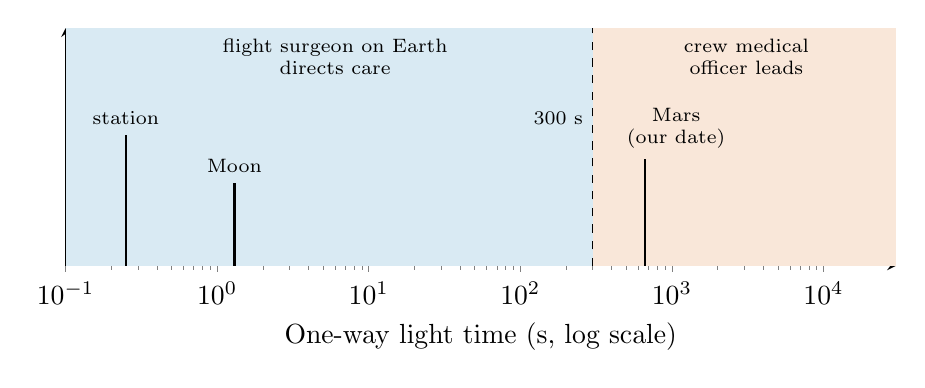
\begin{tikzpicture}
\begin{semilogxaxis}[width=\columnwidth, height=46mm, xmin=0.1, xmax=30000, ymin=0, ymax=1, ytick=\empty,
  xlabel={One-way light time (s, log scale)}, axis lines=left, clip=false]
\fill[oiblue!15] (axis cs:0.1,0) rectangle (axis cs:\numCrewFirstAtS,1);
\fill[oiverm!15] (axis cs:\numCrewFirstAtS,0) rectangle (axis cs:30000,1);
\node[align=center, font=\scriptsize] at (axis cs:6,0.88) {flight surgeon on Earth\\directs care};
\node[align=center, font=\scriptsize] at (axis cs:3100,0.88) {crew medical\\officer leads};
\draw[thick] (axis cs:\numStationOneWayS,0) -- (axis cs:\numStationOneWayS,0.55)
  node[above, font=\scriptsize]{station};
\draw[thick] (axis cs:\numMoonOneWayS,0) -- (axis cs:\numMoonOneWayS,0.35)
  node[above, font=\scriptsize]{Moon};
\draw[thick] (axis cs:\numMarsOneWayS,0) -- (axis cs:\numMarsOneWayS,0.45)
  node[above, font=\scriptsize, align=center, xshift=4mm]{Mars\\(our date)};
\draw[dashed] (axis cs:\numCrewFirstAtS,0) -- (axis cs:\numCrewFirstAtS,1)
  node[pos=0.62, left, font=\scriptsize]{\numCrewFirstAtS~s};
\end{semilogxaxis}
\end{tikzpicture}
\caption{Who leads care, by one-way light time (log scale). The dashed line is the \numCrewFirstAtS~s switch, a design choice. With no link at all the crew act alone.}
\label{fig:authority}
\end{figure}


\paragraph{Can Earth answer first?}
The same arithmetic decides whether Earth can help with a falling reading. Let $T$ be the time left, in seconds, before the reading reaches its red line (Section~\ref{sec:methods}, Equation~\ref{eq:timeleft}). An answer from Earth arrives at the earliest $R$ seconds after the report leaves, so Earth can answer before the red line only if
\begin{equation}\label{eq:earthfirst}
  R = 2\,\Delta t < T .
\end{equation}
The ship makes this comparison in three steps: it computes $T$ from the readings, takes $R$ from the light time for the current stop, and writes the result of $R < T$ into the warning. At Mars on our date $R = \numMarsRoundTripS$~s. The ship states a time left only when $T \le \numHorizonS$~s, because it stays quiet when the red line is further away than that, so every stated $T$ is shorter than $R$ and the comparison always fails. The ship therefore tells the CMO, in one sentence, that Earth's answer would come too late, and the report still leaves for Earth.

\paragraph{Role-based views.}
Watching every reading puts one person's health record in front of the whole crew unless the screens are shaped. The crew console says who is looking in a request header. With no viewer named, the medical station sees every record. The CMO sees every record. Any other crew member sees their own record in full, a name card for each crewmate, and a short notice if a crewmate has an SOS, without the readings behind it. These are role-based views and not authentication: nothing in the system proves who the viewer is, and anyone who can send requests to the ship can name any viewer. They show the intended rule for who reads what; they do not enforce it.

\paragraph{Implementation.}
The ship and the Earth API are a Flask application with SQLAlchemy over SQLite or PostgreSQL. The crew and Earth consoles are a Next.js application that polls the API once a second. Both run in Docker and on Google Cloud Run. No language model is called while a request is handled, and the rules need no outside service: the one outside call, to Horizons for the light time, is cached for the day and falls back to stored values, so the rules keep working with no link. The backend has \numTestCount~automated tests, all of which pass on the commit described here; they cover the rules, the link and its delays, the wall between ship and Earth, and the field names the consoles build against. The crew's month of vital signs and the scripted demo story are simulated, generated from a fixed seed and labelled as simulated on screen. The only real physiological data in this paper are the public research recordings in Section~\ref{sec:methods}, all from volunteers on Earth.

\section{Methods}\label{sec:methods}
% Outline row: methods.tex. Figure 3, the equations, Table 3, datasets with licences, protocol, statistics.

% Figure 3. The three questions LIGHTTIME asks of every reading, in order.
\begin{figure}[t]\centering
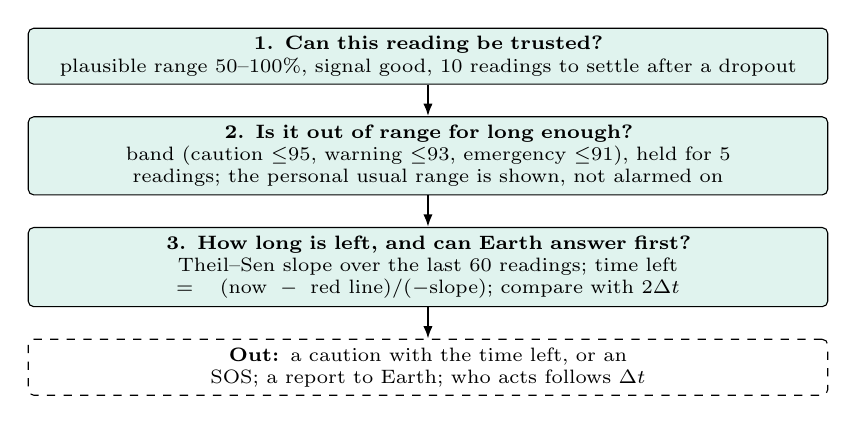
\begin{tikzpicture}[font=\scriptsize, node distance=4mm,
  q/.style={draw, rounded corners=2pt, fill=oigreen!12, align=center, text width=0.82\columnwidth, inner sep=3pt},
  outbox/.style={draw, dashed, rounded corners=2pt, align=center, text width=0.82\columnwidth, inner sep=3pt},
  arr/.style={-{Latex[length=1.6mm]}, thick}]
\node[q] (trust) {\textbf{1. Can this reading be trusted?}\\plausible range \numPlausibleSpoTwoLow--\numPlausibleSpoTwoHigh\%, signal good, \numSettleN{} readings to settle after a dropout};
\node[q, below=of trust] (usual) {\textbf{2. Is it out of range for long enough?}\\band (caution $\le$\numSpoTwoCaution, warning $\le$\numSpoTwoWarning, emergency $\le$\numSpoTwoEmergency), held for \numSustainN{} readings; the personal usual range is shown, not alarmed on};
\node[q, below=of usual] (left) {\textbf{3. How long is left, and can Earth answer first?}\\Theil--Sen slope over the last \numWindowN{} readings; time left $=(\text{now}-\text{red line})/(-\text{slope})$; compare with $2\Delta t$};
\node[outbox, below=of left] (act) {\textbf{Out:} a caution with the time left, or an SOS; a report to Earth; who acts follows $\Delta t$};
\draw[arr] (trust) -- (usual); \draw[arr] (usual) -- (left); \draw[arr] (left) -- (act);
\end{tikzpicture}
\caption{The order in which the ship checks a reading. Each step can stop a false alarm before the next one runs.}
\label{fig:pipeline}
\end{figure}


LIGHTTIME asks three questions of every reading, in a fixed order (Figure~\ref{fig:pipeline}): can it be trusted, is it out of range for long enough to matter, and if it is still in range but falling, how long is left. Each step can stop a false alarm before the next runs. We describe blood oxygen saturation (SpO$_2$), the one vital sign that both raises alarms and carries a trend. Table~\ref{tab:notation} lists every symbol with its meaning and unit, and Table~\ref{tab:params} lists every setting with its value and source.

\begin{table}[t]\centering\footnotesize
\caption{Notation. Readings arrive one a second, so a reading index is also a time in seconds. ``pts'': percentage points of SpO$_2$.}\label{tab:notation}
\setlength{\tabcolsep}{3pt}
\begin{tabular}{@{}L{0.25\columnwidth}L{0.53\columnwidth}L{0.16\columnwidth}@{}}\toprule
Symbol & Meaning & Unit \\ \midrule
$d$ & path length from Earth to the ship & km \\
$c$ & speed of light, \numSpeedOfLightKmS & km\,s$^{-1}$ \\
$\Delta t$ & one-way light time & s \\
$R$ & round trip, $2\Delta t$; earliest reply & s \\
$\tau$ & delay at which the CMO leads & s \\
$t_\text{sent}$, $t_\text{lands}$, $t_\text{now}$ & wall-clock send, landing and display times of a message & s \\
$x_t$ & SpO$_2$ reading at second $t$ & \% \\
$g_t$ & sensor signal-quality flag & true/false \\
$c_t$ & reading $t$ is clean & true/false \\
$L, H$ & lowest and highest plausible SpO$_2$ & \% \\
$N_\text{settle}$ & readings to wait after an unclean one & readings \\
$b(x)$ & band of a reading: 0 normal to 3 SOS & level \\
$N_\text{sus}$ & readings a band must hold & readings \\
$\ell_t$ & level held at second $t$ & level \\
$P_{\numUsualLowPct}, P_{\numUsualHighPct}$ & ends of the person's usual range & \% \\
$W$, $n$ & window length; clean readings in it & readings \\
$M$ & pairs of readings, $n(n-1)/2$ & pairs \\
$\hat\beta$ & Theil-Sen slope & pts\,s$^{-1}$ \\
$N_-, N_+$ & pairs whose slope is negative, positive & pairs \\
$A$ & agreement: Kendall's tau, sign reversed & none \\
$\tilde x$ & current level & \% \\
$r$ & red line, the SOS limit & \% \\
$T$ & time left before the red line & s \\
$n_\text{min}$, $D_\text{min}$, $A_\text{min}$, $T_\text{max}$ & gates on $n$, on the fall, on $A$ and on $T$ & Table~\ref{tab:params} \\
\bottomrule
\end{tabular}
\end{table}

\paragraph{Trust.}
Let $x_t$ be the reading at second $t$ and $g_t$ the sensor's signal-quality flag. A reading is clean when it is plausible and the signal is good:
\begin{equation}\label{eq:clean}
  c_t = \bigl[\, L \le x_t \le H \,\bigr] \wedge g_t ,
\end{equation}
with $L = \numPlausibleSpoTwoLow$\% and $H = \numPlausibleSpoTwoHigh$\%. The bracket is true when the inequality holds, and $\wedge$ is logical and. An SpO$_2$ outside that range is a dropout, not a measurement. A reading with a poor signal is never judged and raises a ``check your sensor'' notice instead. After any unclean reading, nothing can alarm for the next $N_\text{settle} = \numSettleN$ readings, because a probe that has just been put back on reads low for a few seconds. A reading is therefore judged only when it and the $N_\text{settle}$ readings before it are all clean, $c_t \wedge c_{t-1} \wedge \dots \wedge c_{t-N_\text{settle}}$. The public recordings carry no signal-quality flag, so in the replay $g_t$ is true for every reading and only the plausible range applies.

\paragraph{Bands held for a run of readings.}
The band of a reading follows SpO$_2$ Scale~1 of the NEWS2 chart~\cite{rcp2017news2}:
\begin{equation}\label{eq:band}
  b(x) = \begin{cases}
    3 & x \le \numSpoTwoEmergency\%, \\
    2 & x \le \numSpoTwoWarning\%, \\
    1 & x \le \numSpoTwoCaution\%, \\
    0 & \text{otherwise.}
  \end{cases}
\end{equation}
The rows are read from the top, so a reading of \numSpoTwoEmergency\% or less is band 3 even though it also satisfies the lower rows. The levels are named caution (1), warning (2) and emergency, or SOS (3). NEWS2 adds the scores of six physiological parameters before it decides a response; LIGHTTIME acts on the single sign, so its tiers borrow the NEWS2 cut-offs but do not use the score. A level counts only when it holds for the last $N_\text{sus} = \numSustainN$ readings from the same sensor, each clean:
\begin{equation}\label{eq:hold}
  \ell_t = \max\bigl\{ s : c_{t-k} \wedge b(x_{t-k}) \ge s \ \text{for}\ k = 0, \dots, N_\text{sus}-1 \bigr\}.
\end{equation}
In words, $\ell_t$ is the worst band that each of the last \numSustainN{} readings reached; one reading in a better band, or one unclean reading, among them lowers it. An SOS is the moment $\ell_t$ first reaches 3, and it sends a report to Earth on its own. Two further rules shape the alarms in the running ship but play no part in the replay below: a number typed by a person is judged at once but can never rise above a warning, and after a person clears an alert, the same alert stays quiet for \numQuietS~s unless it gets worse.

\paragraph{The person's usual range.}
For each person the ship keeps the range from $P_{\numUsualLowPct}$ to $P_{\numUsualHighPct}$, the \numUsualLowPct st and \numUsualHighPct th percentiles of their clean sensor readings over the last \numUsualHours~hours. Readings marked as exercise are left out, and the range is computed only once at least \numUsualMinReadings{} readings remain; it is refreshed every \numUsualRefreshS~s. Because the ends are percentiles rather than the lowest and highest readings, a few stray readings cannot set the range. The range is shown on the crew card and sent to Earth with every report. It raises no alarm.

\paragraph{Time left.}
A fixed band fires only once the number is already bad, so the third question looks ahead. It takes six steps.

\emph{Step 1, the window.} Take the last $n \le W$ clean readings $x_1, \dots, x_n$, with $W = \numWindowN$. Because readings are one second apart, the index of a reading is its time in seconds.

\emph{Step 2, the slope.} The slope is the Theil-Sen estimate, the median of the slopes between every pair of readings~\cite{theil1950,sen1968}:
\begin{equation}\label{eq:theilsen}
  \hat\beta = \operatorname*{median}_{1 \le i<j \le n} \frac{x_j - x_i}{j - i}.
\end{equation}
Each pair gives a rise over a run, in percentage points per second, and $\hat\beta$ is the middle of the $M = n(n-1)/2$ values; for a full window $M = \numWindowPairs$. When $M$ is even the code takes the larger of the two middle values. We use this estimate because a minority of wild readings cannot pull it far, where one bad point can ruin a least-squares line~\cite{rousseeuw1987}.

\emph{Step 3, the agreement.} Noise always has some slope, so we also measure how consistently the readings fall. With $N_-$ and $N_+$ the numbers of pairs whose slope is negative and positive,
\begin{equation}\label{eq:agreement}
  A = \frac{N_- - N_+}{M},
\end{equation}
which is Kendall's rank correlation between time and reading with the sign reversed~\cite{kendall1938}. $A = 1$ when every pair falls, $A = 0$ when as many pairs rise as fall, and pairs with equal readings count in neither.

\emph{Step 4, the current level.} The current level $\tilde x$ is the median of the last \numNowMedianN{} readings, so one odd reading cannot move it.

\emph{Step 5, the time left.} With red line $r = \numSpoTwoEmergency$\%, the SOS limit of Equation~\ref{eq:band}, the time left is the remaining gap divided by the rate at which it closes:
\begin{equation}\label{eq:timeleft}
  T = \frac{\tilde x - r}{-\hat\beta}\quad\text{seconds}.
\end{equation}
The numerator is in percentage points and the denominator in percentage points per second, so $T$ is in seconds.

\emph{Step 6, the gates.} The ship raises a caution with $T$ attached only when all of the following hold: $n \ge n_\text{min} = \numMinReadings$; $A \ge A_\text{min} = \numMinAgreement$; the fitted line falls at least $D_\text{min} = \numMinDrop$ points across the window, that is $-\hat\beta\,(n-1) \ge D_\text{min}$; $\tilde x > r$; and $T \le T_\text{max} = \numHorizonS$~s. A slow drift that fails the last test is left to the fixed bands. The ship then makes the comparison $R < T$ of Equation~\ref{eq:earthfirst} and freezes it into the report, so Earth later sees what the ship knew when it spoke.

\emph{Worked example.} Take five readings one second apart: \numWorkedReadingOne, \numWorkedReadingTwo, \numWorkedReadingThree, \numWorkedReadingFour{} and \numWorkedReadingFive\%. With $n = \numWorkedN$ there are $M = \numWorkedPairs$ pairs. Every pair falls, so $A = \numWorkedAgreement$. The middle of the \numWorkedPairs{} sorted pair slopes is $\hat\beta = \numWorkedSlope$ points per second. The current level is the median of the five readings, $\tilde x = \numWorkedLevel$\%, which leaves a gap of $\tilde x - r = \numWorkedGap$ points to the red line. Equation~\ref{eq:timeleft} then gives $T = \numWorkedGap / \bigl(-(\numWorkedSlope)\bigr) = \numWorkedTimeLeftS$~s. In the ship these five readings would not yet raise a warning: $n = \numWorkedN$ is below $n_\text{min} = \numMinReadings$, and the fitted fall across the window, $-\hat\beta\,(n-1) = \numWorkedDrop$ point, is below $D_\text{min} = \numMinDrop$. The example shows the arithmetic only.

\begin{table}[t]\centering\footnotesize
\caption{Every setting LIGHTTIME uses, its value and where it comes from. ``LOO'' marks the three settings chosen by the leave-one-recording-out check.}\label{tab:params}
\setlength{\tabcolsep}{3pt}
\begin{tabular}{@{}L{0.37\columnwidth}L{0.27\columnwidth}L{0.30\columnwidth}@{}}\toprule
Setting & Value & Source \\ \midrule
Plausible SpO$_2$, $L$ to $H$ & \numPlausibleSpoTwoLow\% to \numPlausibleSpoTwoHigh\% & \texttt{limits.json} \\
Settle after a dropout, $N_\text{settle}$ & \numSettleN{} readings & \texttt{limits.json} \\
Hold for a band, $N_\text{sus}$ & \numSustainN{} readings & \texttt{limits.json} \\
Caution, warning, SOS & $\le$\numSpoTwoCaution, $\le$\numSpoTwoWarning, $\le$\numSpoTwoEmergency\% & NEWS2~\cite{rcp2017news2}, via \texttt{limits.json} \\
Quiet after a clear & \numQuietS~s & \texttt{limits.json} \\
Window, $W$ & \numWindowN{} readings & \texttt{lookahead.py}, LOO \\
Fewest readings for a trend, $n_\text{min}$ & \numMinReadings & \texttt{lookahead.py} \\
Smallest fall across the window, $D_\text{min}$ & \numMinDrop{} points & \texttt{lookahead.py}, LOO \\
Smallest agreement, $A_\text{min}$ & \numMinAgreement & \texttt{lookahead.py}, LOO \\
Readings in the current level & \numNowMedianN & \texttt{lookahead.py} \\
Furthest red line worth a warning, $T_\text{max}$ & \numHorizonS~s & \texttt{lookahead.py} \\
Usual range & $P_{\numUsualLowPct}$ to $P_{\numUsualHighPct}$, \numUsualHours~h, $\ge$\numUsualMinReadings{} readings & \texttt{usual.py} \\
Crew medical officer leads at, $\tau$ & $\Delta t \ge \numCrewFirstAtS$~s & \texttt{modes.py}; our choice after~\cite{rader2013delay} \\
Mars $\Delta t$, 14 Nov 2026 & \numMarsOneWayS~s & Horizons~\cite{giorginiHorizons}, \texttt{lighttime.py} \\
Demo speed-up & $\times$\numSpeedup & \texttt{link.py} \\
Heart-rate adviser limit (offline), $\lambda$ & \numHrLimitBpm~bpm & learned, \texttt{hr\_normal.json} \\
\bottomrule
\end{tabular}
\end{table}

\paragraph{Datasets.}
Three public datasets were used, all recorded from volunteers on Earth. The University of Washington induced-hypoxemia data~\cite{hoffman2022oximetry} hold \numUwEvents{} recordings of healthy adults who breathed lowered-oxygen gas mixes in a clinical laboratory for \numUwMinutesMin{} to \numUwMinutesMax{} minutes each; we use the reference finger oximeter (Masimo Radical-7) column, one reading a second, unchanged (MIT licence). From the PhysioNet Apnea-ECG Database~\cite{penzel2000apnea,physionetApnea,goldberger2000physionet} we use the SpO$_2$ channel of two overnight records, the control night \texttt{c01r} and the sleep-apnoea night \texttt{a01r}, reduced to one reading a second by taking the first sample of each second; a value of zero marks the probe off (Open Data Commons Attribution License v1.0). PPG-DaLiA~\cite{reiss2019ppg,ppgDaliaData} gives wrist heart rate, one value a second, from \numHrPeople{} people going through sitting, desk work, walking, cycling, stairs and other daily activities (CC BY 4.0). None of the recordings contains a medical emergency.

\paragraph{Replay protocol.}
Each SpO$_2$ recording was played one reading a second through the function \texttt{play()} in \nolinkurl{scripts/check_spo2_rules.py}. That loop calls the ship's own band function, settle and hold counts from \texttt{limits.json}, and the ship's own trend function (\texttt{lookahead.falling}). It replaces the ship's database with lists, so the alert bookkeeping is re-implemented rather than shared. The SOS time of a recording is the first second at which \numSustainN{} clean readings in a row sit in the emergency band. A trend warning is the first second at which the time-left gates pass; a later one counts as new only after a minute without one. In the running ship the trend rule raises its own caution only while no band is held; once a caution or warning band is held, the time left is shown beside that open alert instead. The replay counts a trend warning in either case, so for each one we also report whether a band was already held, and whether any trend warning came before the band rule's first caution. For each low-oxygen recording we report the last warning before the SOS, the lead (SOS time minus warning time) and the time left the ship stated at that warning. On the control night we count false SOS alarms and trend warnings three times: with every number believed, with impossible numbers removed, and with the settle count added as well. On the apnoea night we count how often a trend warning came within \numApneaLookbackS~s before an SOS.

\paragraph{Choosing the time-left settings.}
The window, smallest fall and smallest agreement were chosen on the same \numUwEvents{} recordings, so we checked the choice by leaving each recording out in turn. The grid held \numGridSize{} settings: window \numGridWindowShort{} or \numGridWindowLong{} readings, smallest fall \numGridDropLow, \numMinDrop{} or \numGridDropHigh{} points, and smallest agreement \numGridAgreeLow, \numMinAgreement{} or \numGridAgreeHigh. A setting was allowed only if it raised at most \numGridMaxControlWarnings{} trend warnings on the control night. For each held-out recording, we took the allowed setting that warned first on the most of the other recordings, broke ties by the longest median lead, and applied it to the held-out one. The control night was used in every round and is not held out.

\paragraph{The offline heart-rate adviser.}
NEWS2 heart-rate bands raised alarms on most of the healthy PPG-DaLiA volunteers during ordinary desk work (\nolinkurl{data/ppg_dalia/README.md}), so heart rate raises no alarm in LIGHTTIME. Instead we fitted one small statistical model offline. For person $p$ in activity $a$, the expected heart rate in beats a minute is
\begin{equation}\label{eq:hr}
  \hat h_{p,a} = m_{p,\text{rest}} + \operatorname*{median}_{q}\bigl(m_{q,a} - m_{q,\text{rest}}\bigr),
\end{equation}
where $m_{p,a}$ is the median rate of person $p$ in activity $a$ and the median runs over the training people $q$. The first term is the person's own resting rate and the second the typical rise for that activity. The limit $\lambda$ is the \numHrLimitPercentile th percentile of $|h - \hat h|$ over the training people, where $h$ is the measured rate, and a minute is flagged when \numHrSustainS{} seconds in a row lie more than $\lambda$ from $\hat h$. The model was fitted \numHrPeople{} times, each time leaving one person out and testing on that person, against a gate fixed before the run: at most \numHrGateMinPerH{} flagged minute an hour on any held-out person. It is not connected to the ship.

\paragraph{Statistics.}
All results are descriptive: counts, medians and ranges, reported for every event. With \numUwEvents{} events, no hypothesis test or confidence interval would be informative, and none is given. Every number in this paper is written by \texttt{scripts/paper\_numbers.py} from the code and the recordings and read into the text as a macro.

\section{Results}\label{sec:results}
% Outline row: results.tex. Table 2, Figures 4 and 5, the control night, the held-out result,
% the heart-rate adviser. Description only; interpretation is in the Discussion.

\begin{table}[t]\centering\footnotesize
\caption{Each induced low-oxygen recording replayed through the ship's rules. Warning: the last trend warning before the SOS. SOS: the first second with \numSustainN{} clean readings in a row at or below \numSpoTwoEmergency\%. Lead: SOS minus warning. Predicted left: the time left the ship stated at the warning. All times in seconds from the start of the recording.}\label{tab:events}
\setlength{\tabcolsep}{4pt}
% Written by scripts/paper_numbers.py. Do not edit by hand.
\begin{tabular}{@{}lrrrr@{}}\toprule
Recording & Warning (s) & SOS (s) & Lead (s) & Predicted left (s)\\ \midrule
100001 & 162 & 321 & 159 & 142 \\
100002 & 235 & 341 & 106 & 56 \\
100003 & 138 & 236 & 98 & 87 \\
100004 & 221 & 317 & 96 & 58 \\
100005 & 112 & 180 & 68 & 84 \\
100006 & 114 & 128 & 14 & 26 \\
\bottomrule\end{tabular}

\end{table}

\paragraph{Low-oxygen recordings.}
Table~\ref{tab:events} lists every event. In all \numUwEvents{} recordings the SpO$_2$ reached the emergency band, and in \numUwWarned{} of the \numUwEvents{} the ship raised a trend warning before the SOS. The lead ranged from \numUwMinLeadS{} to \numUwMaxLeadS~s, with a median of \numUwMedianLeadS~s (Figure~\ref{fig:evidence}, left). The counted warning came while the reading was still in the normal band in \numUwWarnNormalBandN{} of the \numUwEvents{} recordings (Figure~\ref{fig:event}). In the other recordings a caution or warning band was already held, so the fixed bands had already raised an alert and the warning added the time left to it. A trend warning came before the band rule's first caution in \numUwTrendBeforeCautionN{} of the \numUwEvents.

\begin{figure}[t]\centering
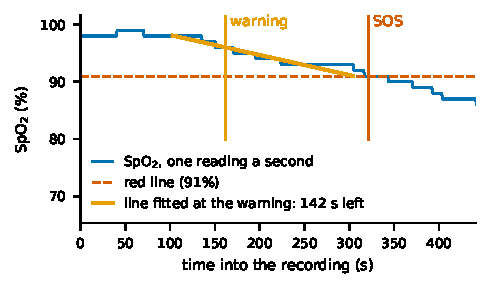
\includegraphics[width=\columnwidth]{figures/timeleft_event.pdf}
\caption{Recording 100001 of the induced low-oxygen data~\cite{hoffman2022oximetry}. The ship warned at the orange line and fitted the orange slope through the readings before it; the SOS (vermilion line) followed when \numSustainN{} readings in a row sat at or below the red line.}
\label{fig:event}
\end{figure}

The time left that the ship stated differed from the lead it actually had by a median of \numUwPredAbsErrMedianS~s and at most \numUwPredAbsErrMaxS~s. The stated time was shorter than the lead in \numUwPredShortN{} recordings and longer in \numUwPredLongN, by at most \numUwPredLongMaxS~s.

\paragraph{Held-out choice of settings.}
Of the \numGridSize{} settings in the grid, \numGridAllowed{} raised at most \numGridMaxControlWarnings{} trend warnings on the control night. In \numHeldoutRoundsShipSetting{} of the \numHeldoutRounds{} leave-one-out rounds, the setting chosen without the held-out recording was the one the ship runs (Table~\ref{tab:params}). Applied to the held-out recordings, the chosen settings warned before the SOS in \numHeldoutWarned{} of \numUwEvents, with a median lead of \numHeldoutMedianLeadS~s, the same as Table~\ref{tab:events}.

\begin{figure}[t]\centering
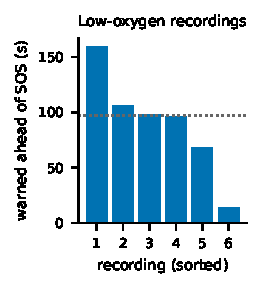
\includegraphics[width=0.49\columnwidth]{figures/lead_times.pdf}\hfill
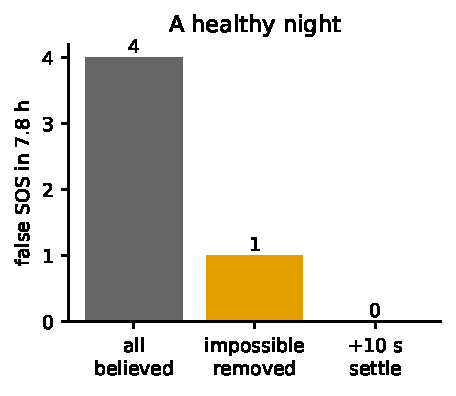
\includegraphics[width=0.49\columnwidth]{figures/false_sos.pdf}
\caption{Left: warning lead before the SOS in each of the \numUwEvents{} low-oxygen recordings, sorted; the dotted line is the median, \numUwMedianLeadS~s. Right: false SOS alarms on a healthy \numControlHours-hour night (Apnea-ECG \texttt{c01r}) with no trust rule, with the plausible-range check, and with the \numSettleN-reading settle count added.}
\label{fig:evidence}
\end{figure}

\paragraph{The healthy night.}
The control record held \numControlHours~hours of plausible SpO$_2$ readings. With every number believed, the band rule raised \numControlFalseSosRaw{} false SOS. Removing impossible numbers left \numControlFalseSosReject, and adding the settle count left \numControlFalseSosSettle{} (Figure~\ref{fig:evidence}, right). With the trend rule switched on, the same night raised \numControlTrendWarnings{} trend warnings. Each was a caution, the lowest level, and sent no SOS, but nothing was wrong with the sleeper, so we count both as false warnings.

\paragraph{The apnoea night.}
On the sleep-apnoea record (\numApneaHours~hours of plausible readings), the band rule raised an SOS \numApneaSosN{} times. A trend warning came within the \numApneaLookbackS~s before the SOS in \numApneaWarnedFirstN{} of them (\numApneaWarnedFirstPct\%), with a median lead of \numApneaMedianLeadS~s. In the rest, the SOS came from the fixed band alone.

\paragraph{The heart-rate adviser.}
Fitted on all \numHrPeople{} people, the adviser's limit was \numHrLimitBpm~beats a minute from the expected rate. Across the \numHrPeople{} leave-one-person-out rounds, the worst held-out person had \numHrWorstFlaggedMinPerH{} flagged minutes an hour, inside the gate of \numHrGateMinPerH. No recording contains an emergency, so this measures only how often it flags healthy people. The adviser is not wired into the ship.

\section{Discussion}\label{sec:discussion}
% Outline row: discussion.tex. Meaning against a 22-minute round trip; design lessons; limits in order of
% weight; ethics. Nothing softened.

\paragraph{What the numbers mean at Mars.}
On our mission date the earliest reply from Earth is \numMarsRoundTripS~s away. The longest lead in the replay was \numUwMaxLeadS~s. So in every low-oxygen event we replayed, no answer from Earth could have arrived before the SOS, and the person who could act in time was the CMO on board. That is the situation the design is built for. At Mars a warning cannot buy time for Earth. What it can do is tell the CMO early, in one sentence, that the call is theirs, while the report travels to Earth for review. The same warnings at the Moon, with a round trip of a few seconds, would leave the flight surgeon time to direct care, and the ship would say so.

The replay also shows what the trend rule did not do. In most recordings a fixed band was already held when the counted warning came, and only in \numUwTrendBeforeCautionN{} of \numUwEvents{} did any trend warning come before the band rule's first caution. On these recordings the trend rule rarely gave an earlier alarm. What it added was a stated deadline that can be set against the round trip. That deadline was off by a median of \numUwPredAbsErrMedianS~s, mostly on the short side. Two effects pull it in opposite directions. The SOS needs \numSustainN{} readings in the red, so it lands a few seconds after the line is crossed, which makes the stated time look short. And early in a fall the \numWindowN-reading window still holds flat readings, so the slope is too shallow and the stated time too long; the fall then steepens. When a fall is faster than the window can follow, the trend rule is silent and the fixed bands catch it, as on the apnoea night, where the trend warning came first for only \numApneaWarnedFirstPct\% of falls.

\paragraph{Design lessons.}
Three choices carried most of the weight. The first is to make authority an explicit rule: who decides is computed from one number, shown on every screen, and covered by tests, rather than left to whoever happens to be watching. The second is trust before trend. On the healthy night the plausibility check and the settle count removed every false SOS before any slope was fitted; a trend fitted to dropouts would have been worse than none. The third is store and forward. The Earth console shows only what has landed, and each report carries answers to the questions a flight surgeon asks first, because at Mars each question costs a round trip. Every alert also prints its reasons (what was seen, the last readings, the rule and the source of the band table) and the same closing line: this is a fixed rule, not a diagnosis, and a person decides. A rule can explain itself in a few lines, which is one reason the project lets no trained model decide (\nolinkurl{docs/adr/0001-rules-decide-learned-models-advise.md}).

\paragraph{Limits.}
We list the limits in order of weight. The first is sample size. There are \numUwEvents{} low-oxygen events, one healthy control night, one apnoea night and \numHrPeople{} people for the heart-rate adviser. The results are counts and medians from a handful of recordings and say nothing about rates in a population. Second, the low oxygen was induced in a laboratory on Earth: volunteers breathed controlled gas mixes while a reference finger oximeter read once a second~\cite{hoffman2022oximetry}. A fall in a spacecraft, from a cabin fault or an illness, may be faster or slower, and a shirt-borne sensor on a moving person will be noisier. Third, the volunteers were healthy, and none of the recordings contains a medical emergency. Fourth, the time-left settings were chosen on the same \numUwEvents{} recordings that test them. Leaving each recording out guards against a lucky choice, and every round picked the same setting, but the grid was small and the control night was shared by every round. Fifth, only blood oxygen carries a trend. Heart rate raises no alarm, and there is no rule for a fast heart at rest, a slow heart in sleep, or a sensor stuck on one value. Sixth, the bands follow NEWS2, a score built for patients in hospital~\cite{rcp2017news2} that has not been validated in spaceflight, and nobody has checked whether its bands suit a healthy crew in a spacecraft cabin; our tiers are inspired by it, nothing more. Seventh, the crew's month of data and the demo story are simulated. Eighth, light time is only the floor of the latency. Relay visibility windows and solar conjunction add to it~\cite{mcbrayer2022delay}, as does the time a person on the ground takes to read and answer; all of these make the true delay longer, so they strengthen the case for crew-led care at Mars rather than weaken it. Ninth, the \numCrewFirstAtS~s switch is our choice, informed by one analog mission~\cite{rader2013delay}. Tenth, we assume the crew wear the shirt for the whole mission. A monitor that records every second of a person's body for years is a large intrusion, and whether it is proportionate to the risk is an open question; in quiet phases, periodic checks may be enough. LIGHT-TIME keeps the raw stream on the ship for \numRecorderHours~hours and sends Earth only reports and daily summaries, but that is a design choice, not a safeguard anyone has tested. Eleventh, we ran no human-factors study: we do not know whether a CMO under stress understands the sentence, trusts it, or acts faster because of it, and the simulator evidence that crews do worse without a flight surgeon~\cite{yule2023crew} is a warning against assuming so. Twelfth, the role-based views are not authentication; anyone who can reach the ship can claim to be anyone. In the hosted demo two gaps remain: the console does not yet send the viewer header, so its screens get the medical station's view, and the routine vitals messages in the ship's outbox carry no crew identifier, so they are not filtered by viewer. Last, the ship's sentence always calls on the CMO, even when the CMO is the patient, a case NASA's CDSS concept of operations plans for~\cite{krihak2021cdss}.

\paragraph{Ethics.}
All physiological data in this paper come from public, de-identified datasets used under their licences (Section~\ref{sec:methods}). We collected no new data from people. Nothing here is a medical device, and none of the wording on the checklists is medical advice.

\section{Conclusion}\label{sec:conclusion}
% Outline row: conclusion.tex. What was shown, at its true size, and what would test it properly.

LIGHT-TIME makes the one-way light time an input to crew health monitoring. The ship computes who must act, Earth or the crew, from the light time for the mission date, and attaches to each falling-trend warning a time left that it compares with the round trip. Replayed through the same rules, \numUwEvents{} public recordings of induced low oxygen were all warned before the SOS, by a median of \numUwMedianLeadS~s, and settings chosen without each recording did as well; on a healthy night the trust rules took false SOS from \numControlFalseSosRaw{} to \numControlFalseSosSettle. Those numbers come from a handful of healthy volunteers on Earth. They show that the parts work together as designed. They do not show that the system would help a crew.

Three steps would test it properly. The first is to run it with a real smart shirt in an analog habitat, with the delay imposed, so the sensors are noisy and the people are busy. The second is an emergency unlock that lets the crew member helping a casualty see that person's full record, logged and reviewed afterwards, since the role-based views now hide it. The third is a study with crews in training, comparing how they handle a falling reading with and without the deadline sentence.

\section*{Availability}
The backend, with the rules, the replay scripts and the tests, is at \url{https://github.com/NASA-space-apps-the-procrastinators/LightTime-backend} (this paper describes commit \texttt{0fa4441} of \texttt{main}, with the paper scripts added for this draft); the consoles are at \url{https://github.com/NASA-space-apps-the-procrastinators/LightTime-frontend}. The repositories are to be made public before this paper is posted. \texttt{python scripts/paper\_numbers.py} writes every number in the text and Table~\ref{tab:events}, and \texttt{python scripts/paper\_figures.py} draws Figures~\ref{fig:event} and~\ref{fig:evidence}. The datasets are available from their publishers~\cite{hoffman2022oximetry,physionetApnea,ppgDaliaData}.

\section*{Use of AI tools}
Claude and Claude Code (Anthropic) were used throughout the project: to plan and write much of the backend code and its tests, to design the time-left rule's settings search, to write the documentation, and to draft this paper. The tools did not decide what the paper claims. Every number in the text is written by a script from the code and the recordings, the tests run against the code, and every reference was checked against its DOI record or the source page on 15 November 2026. Each use is logged in \texttt{AI\_USE.md} in the backend repository. Not every author has yet read this draft.

\section*{Acknowledgements}
We thank the NASA Space Apps Challenge organisers, and the authors of the three public datasets for releasing them. Advisers who commented on the hackathon build will be named here only with their permission.

\section*{Author contributions}
To be agreed by the team before submission.

\bibliographystyle{unsrtnat}
\bibliography{refs}
\end{document}
